\section{Tools \& Tactics}

\begin{frame}[fragile]{Microsoft Exchange Transport Agent}
    \begin{itemize}
        \item Transport agents let you install custom software that is created by Microsoft, by third-party vendors, or by your organization, on an Exchange server \cite{transMicro}
        \item This software can then process email messages that pass through the transport pipeline
        \item Having a single pipeline means that you can have confidence that every message goes is processed in the same way; however it also means that if an attacker can introduce a transport agent, they have access to \emph{every message}
        \item LightNeuron it's the first malware that uses a Transport Agent for malicious purposes
    \end{itemize}
\end{frame}

\begin{frame}[fragile]{LightNeuron components}
    Two main components comprise LightNeuron: 
    \begin{itemize}
        \item a \emph{Transport Agent} that can process and modify all email messages going through the mail server 
        \item a companion 64-bit \emph{Dynamic Link Library (DLL)} containing most of the malicious code.
    \end{itemize}
\end{frame}


\begin{frame}[fragile]{Turla modus operandi}
    A tipical Turla attack chain involves:
    \begin{enumerate}
        \item \textbf{Initial Reconnissance}, usually a basic first-stage malware or a more powerful one if they deem the victim interesting (Metasploit, Carbon or Gazer). Very specific targets
        \item \textbf{Credential Gathering}, they move laterally on the network to collect accounts, using stealthy communications and periodically creating new accounts for persistence
        \item \textbf{Exfiltration}, using an HTTP/email C\&C channel and SATCOM IP addresses to obfuscate the traffic content and destination. 
    \end{enumerate}
    
\end{frame}

\begin{frame}[fragile]{LightNeuron Attack Chain (MITRE ATT\&CK)}
    % The basis of ATT&CK is the set of individual techniques that represent actions that adversaries 
    % can perform to accomplish objectives. Those objectives are represented by the tactic categories
    % the techniques fall under.
    %
    % tattica = obiettivo
    % tecnica = attacco per raggiugnere obiettivo (sfuttare vulnerabilità)
    
    \begin{enumerate}
        \item[1.] \textbf{Initial Acces \& Privilege Escalation}: Valid Accounts using MITM, spreadpishing emails and watering-hole attacks
        \item[2.] \textbf{Execution}: PowerShell script to install Lightneuron components
        \item[3a.] \textbf{Collection}: Automated Collection of both emails and files
        \item[3b.] \textbf{Command \& Control}: email communication using cryptography and steganography
        \item[4.] \textbf{Exfiltration}: Automated and Encrypted exfiltration via C\&C interface with optional night scheduling
    \end{enumerate}
\end{frame}

\begin{frame}[fragile]{Initial Access \& Privilege Escalation}
    \begin{itemize}
        \item Valid Accounts T1078: adversaries may steal the credentials of a 
        specific user or service account using Credential Access techniques
         or capture credentials earlier through social engineering \cite{MitreTechniques}
        \item The attackers must have privileged administrative access to 
        the server in order to start the attack chain 
    \end{itemize}
\end{frame}

\begin{frame}[fragile]{Execution}
    \begin{itemize}
        \item PowerShell T1086: a powershell script is executed
        \item The malicious Transport Agent is a 32-bit Windows DLL developed in .NET
        \item The attackers drop this executable in the Exchange folder located in the 
        Program Files folder.  
    \end{itemize}
\end{frame}

\begin{frame}[fragile]{Execution: Transport Agent Installation}
    Once admin priviledge have been obtained, a PowerShell script is executed to 
    register the DLL as a Transport Agent
    \begin{figure}
        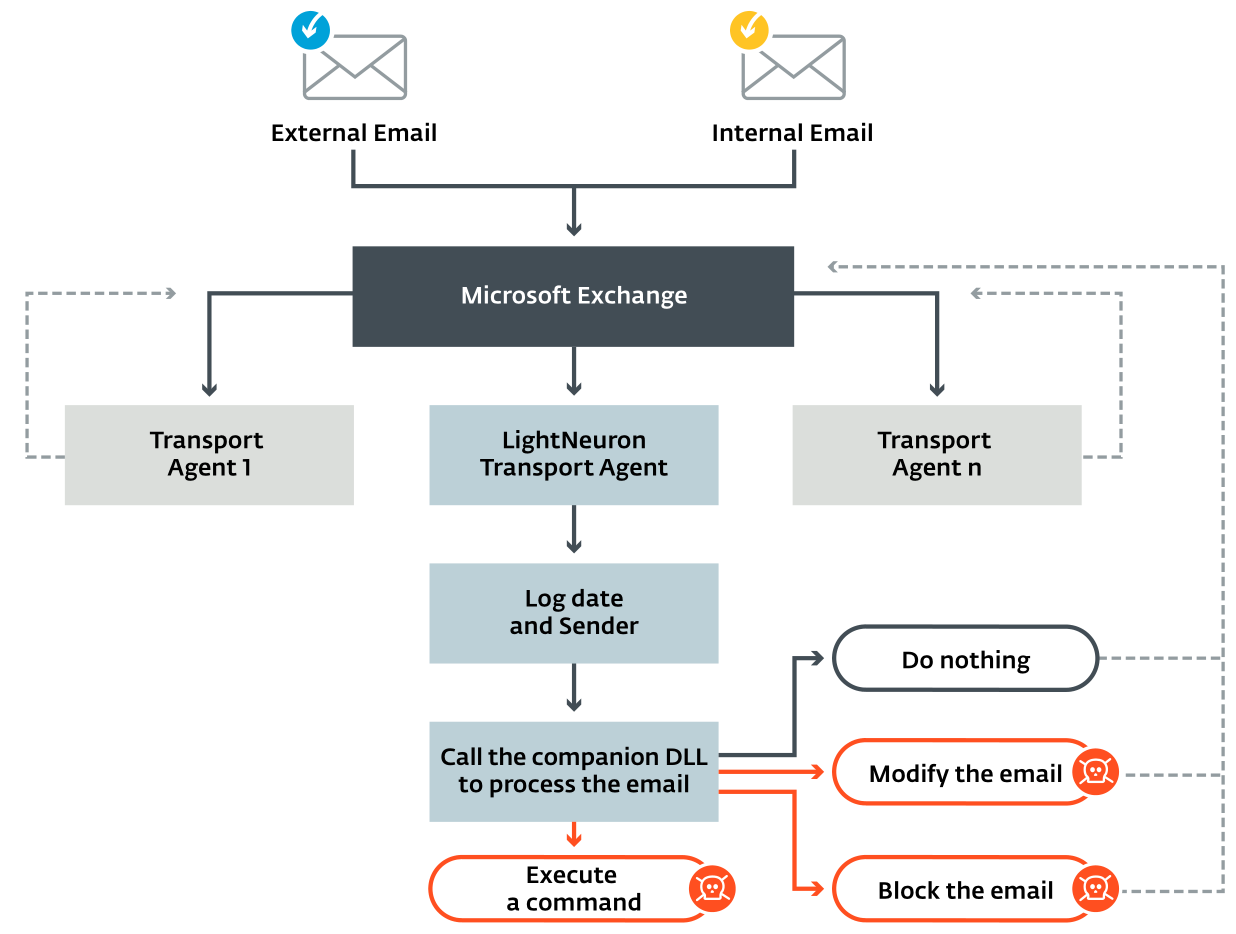
\includegraphics[width=8cm]{figures/transport_agent.PNG}
        \caption{LightNeuron Transport Agent}
    \end{figure}
\end{frame}

\begin{frame}[fragile]{Execution: Companion Dynamic Link Libray}
    \begin{itemize}
        \item The companion DLL is a 64-bit Windows DLL developed in C
        \item When the Transport Agent loads the DLL, 
        the DLL’s main function performs various initialization tasks.
        \item After initail decription operations, it decrypts 
        the configuration file stored in \texttt{\%tmp\%/winmail.dat}; 
        this filename has been chosen to hide their configuration file in plain sight
    \end{itemize}
\end{frame}

\begin{frame}[fragile]{The Configuration Files}
    \begin{itemize}
        \item The configuration file \texttt{winmail.dat} contains various parameters
        \item An interesting one is \texttt{CONFIG\_FILE\_NAME}
        \item Once decrypted, this second configuration file contains the rules used to process the emails.
    \end{itemize}
\end{frame}

\begin{frame}[fragile]{Configuration File Rule System}
    \begin{itemize}
        \item The second configuration file contains several class nodes, each one corresponding to a different function 
        (aka handler) implemented in the DLL. 
        \item Each class node contains a set of rules describing conditions using the logical operators AND and OR. 
        \item At the end of the file is the mapping of the class names with the name of the functions in the DLL.
    \end{itemize}
    \begin{figure}
        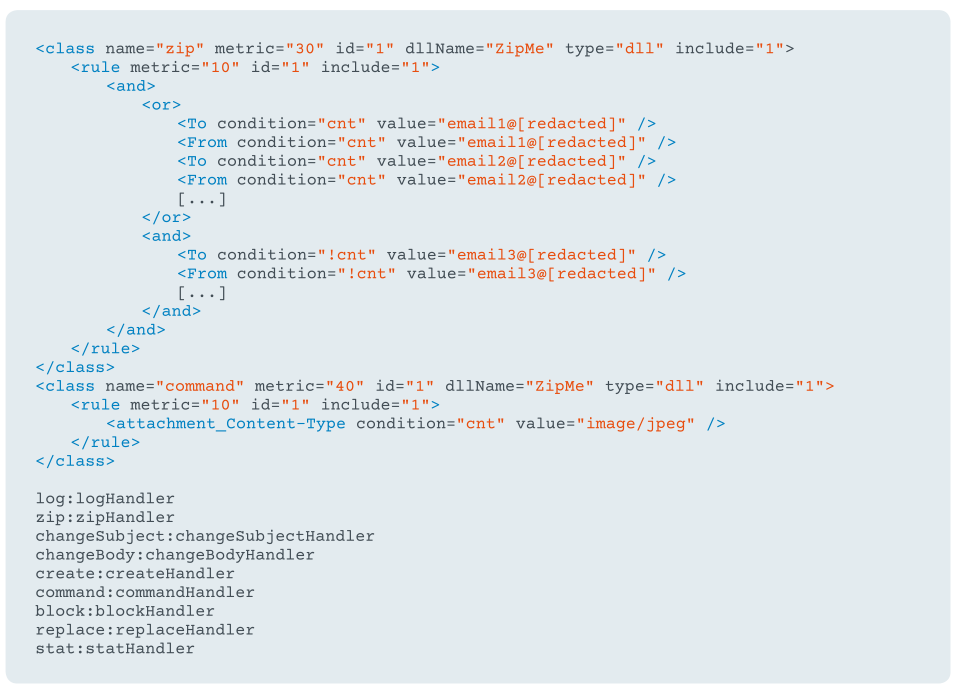
\includegraphics[width=7cm]{figures/rule_file.PNG}
    \end{figure}
\end{frame}

\begin{frame}[fragile]{Configuration File Rule System condt}
    \begin{itemize}
        \item These rules are applied to every email processed by the DLL
        \item This configuration is highly flexible
        \item There are eleven different handlers implemented in the DLL 
    \end{itemize}
\end{frame}